\section{Plateformes de développement}\label{sec:etat_art-802.15.4}
\renewcommand{\rightmark}{Plateformes de développement}
\subsection*{Zolertia RE-Mote}
Pour ce mémoire, la plateforme Zolertia RE-Mote revision B(Fig.~\ref{fig:state-zolertia}) est utilisée.

Cette plateforme, basée sur un system on chip (SoC) CC2538 ARM Cortex-M3, a été conçue par des universités et des industriels dans le but de permettre aux chercheurs et makers de développer des applications IoT et des objets connectés.

Le Zolertia RE-Mote a été choisi car elle est équipée de deux radios compatibles IEEE 802.15.4,
permet une consommation électrique faible et possède de nombreux pins de connexion qui peuvent être utilisés pour y connecter des capteurs, actuateurs, radios, etc.

Le prix du consturcteur pour cette plateforme est de 93,95€~\cite{zolertia-remote:shop}.

\begin{figure}[H]
    \centering
    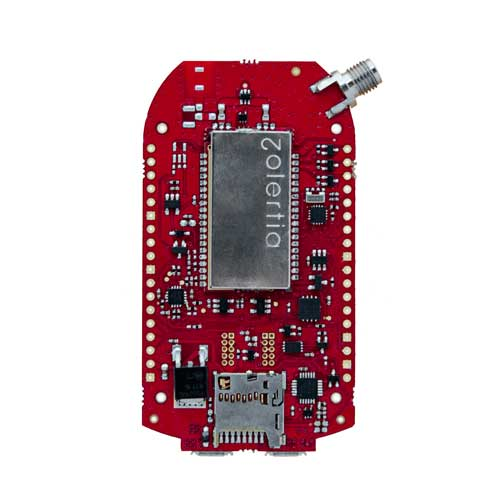
\includegraphics[scale=0.5]{res/remote-zolertia.jpg}
    \caption{Zolertia RE-Mote révision B~\cite{zolertia-remote:shop}.}
    \label{fig:state-zolertia}
\end{figure}

La table~\ref{tb:state-spec} reprend les principales spécifications du Zolertia RE-Mote rev.b et sa table ... la consommation électique.%TODO datasheet ???

\begin{table}[H]
    \centering
    \begin{tabular}{|c|c|}
        \hline
        \rowcolor{lightgray}
        Element            & Spécification\\
        \hline
        Radio              & Deux radios IEEE 802.15.4 à 2.4 GHz et 863-950 MHz\\
        \hline
        CPU                & ARM\textsuperscript{\tiny\textregistered} Cortex\textsuperscript{\tiny\textregistered} -M3 jusqu'à 32 MHz\\
        \hline
        RAM                & 32 KB (16 KB pour tous les Power Modes)\\
        \hline
        Flash programmable & 512KB\\
        \hline
        I/O                & RGB led, boutton user et reset, USB 2.0 à 12Mbps, Real-Time Clock\\
        \hline
    \end{tabular}
    \caption{Spécifications du Zolertia RE-Mote rev.b~\cite{zolertia-remote:datasheet}.}
    \label{tb:state-spec}
\end{table}

\subsection*{RN2483}

\subsection*{Raspberry Pi}

